\documentclass{article}

% Language setting
% Replace `english' with e.g. `spanish' to change the document language
\usepackage[english]{babel}

% Set page size and margins
% Replace `letterpaper' with `a4paper' for UK/EU standard size
\usepackage[letterpaper,top=2cm,bottom=2cm,left=3cm,right=3cm,marginparwidth=1.75cm]{geometry}

% Useful packages
\usepackage{amsmath}
\usepackage{graphicx}
\usepackage[colorlinks=true, allcolors=blue]{hyperref}
\usepackage{algorithm}
\usepackage{algorithmic}
\usepackage{array}
\usepackage{graphicx}
\usepackage{subfig}
\usepackage[section]{placeins}

\title{Heuristic Optimization Methods
\\ Capacitated Vehicle Routing Problem with Time Windows}

\author{Čubek Matej & Paradžik Berislav}

\begin{document}
\maketitle

\clearpage

\tableofcontents

\clearpage

\section{Problem description}
The problem described in the text is the capacitated vehicle routing with time windows (CVRPTW) problem, which is a variant of the vehicle routing problem (VRP). It involves finding a set of routes for a fleet of vehicles serving customers from a depot while considering capacity and time window constraints. In this problem, the vehicles have a limited capacity, and customers must be served within their specified time windows and the working hours of the depot. The problem instances include information about the number of vehicles, the capacity of each vehicle, and data about each customer such as their coordinates, resource demands, schedule horizon, and the duration of the service time.

The problem defines the following constrains:
\begin{enumerate}
  \item Each customer is served by exactly one vehicle/route, with the resource amounts
  \item The demand on each route must not exceed the capacity of the vehicle.
  \item The vehicle servicing a certain customer must arrive at the customer location
within the interval given for that customer. The duration of the service can
exceed the interval.
\item Each vehicle starts and finishes its route in node 0 (customer 0 location; depot),
within the time interval given for customer 0.
\end{enumerate}


\section{Description of the implemented heuristic algorithm}
Greedy algorithm is used for construction phase, for local search is used Large Neighbourhood Search. Large Neighbourhood Search randomly removes n customers from solution and then puts them back in random routes to optimal positions. New solution is not accepted if it is worse or does not fulfil all constraints(except maximum number of routes).

\begin{center}
\begin{tabular}{ | m{15em} | m{30em} | }  
  \hline
  Solution representation & List of routes, each route contains list of customers in exact order they are served. Each customer is served by exactly one vehicle/route. \\ 
  \hline
  Objective function & min(numberOfRoutes, totalDistance), $ \infty $  if constraints are not meet. For example, when comparing 2 solutions solution1 and solution2, better solution is one that has lower number of routes, if both solution have same number of routes, better solution is the one which has lower total distance. \\
  \hline
  Fitness function(score) & $ min(numberOfRoutes^{alpha} + getAllRoutesTime^{beta}), alpha = 3, beta = 1 $ \\ 
  \hline
  Construction of an initial solution & Greedy Algorithm \\ 
  \hline
  Termination criterion & Time constrain, in this project, time constrains were 1 minute, 5 minute and 6 hours. \\ 
  \hline
\end{tabular}
\end{center}

\clearpage

\section{Pseudocode of the implemented algorithm}

\begin{algorithm}
\caption{Greedy Algorithm - construction phase}
    \begin{algorithmic} 
    \STATE $leftCustomers \leftarrow loadAllCustomers()$
    \STATE $routes \leftarrow new List()$
    \STATE $depot \leftarrow leftCustomers.removeFirst()$
    \WHILE{$not leftCustomers.isEmpty()$}
        \STATE $route \leftarrow new Route(vehicleInstance.capacity())$
        \STATE $lastCustomer = depot$
        \STATE $route.addCustomerToRouteEnd(depot)$
        \WHILE{$not leftCustomers.isEmpty()$}
            \STATE $lastCustomerFinal \leftarrow lastCustomer$
            \STATE $potentialNextStop = leftCustomers.stream().filter(satisfy all route constraints).findClosest()$
            \IF{$potentialNextStop is None$}
                \STATE $break$
            \ENDIF
            \STATE $lastCustomer \leftarrow potentialNextStop$
            \STATE $route.addCustomerToRouteEnd(lastCustomer)$
            \STATE $leftCustomers.remove(lastCustomer)$
        \ENDWHILE
        \STATE $route.addCustomerToRouteEnd(depot)$
        \STATE $routes.add(route)$
    \ENDWHILE
    \RETURN routes
\end{algorithmic}
\end{algorithm}

\begin{algorithm}
\caption{Neighbourhood Iterator - function next}
\textbf{Input} $solution, minCustomersToRemove, maxCustomersToRemove$
    \begin{algorithmic} 
    \STATE $random \leftarrow new Random()$ 
    \STATE $numberOfCustomersToRemove = random.nextInt(minCustomersToRemove, maxCustomersToRemove + 1)$ 
    \STATE $customersToRemove = pickRandomCustomersToRemove(numberOfCustomersToRemove)$
    \STATE $routesCopy = copyRoutes()$
    \STATE $routesWithRemovedCustomers = removeCustomersFromRoute(routesCopy, customersToRemove)$
    \STATE $newRoutes = addCustomersToRandomRouteInOptimalList(routesWithRemovedCustomers, customersToRemove)$
    \RETURN $newRoutes$
\end{algorithmic}
\end{algorithm}

\begin{algorithm}
\caption{Large Neighbourhood Search Algorithm}
    \begin{algorithmic} 
    \STATE $timer \leftarrow loadTimer()$ 
    \STATE $neighbourhoodIteratorCreator \leftarrow new loadNeighbourhoodIteratorCreator()$ 
    \STATE $incumbent \leftarrow GreedyAlgorithm()$
    \STATE $incumbentScore \leftarrow new List()$
    \WHILE{$timer.isActive()$}
        \STATE $neighbourhoodIterator = neighbourhoodIteratorCreator.apply(incumbent, timer)$
        \WHILE{$neighbourhoodIterator.hasNext()$}
            \STATE $neighbour = neighbourhoodIterator.next(solution, minCustomersToRemove, maxCustomersToRemove)$
            \STATE $neighbourScore = objectiveFunction.score(neighbour)$
            \IF{$neighbourScore < incumbentScore$}
                \STATE $incumbent \leftarrow neighbour$
                \STATE $incumbentScore \leftarrow neighbourScore$
                \STATE $break$
            \ENDIF
        \ENDWHILE
    \ENDWHILE
    \RETURN incumbent
\end{algorithmic}
\end{algorithm}

\clearpage

\section{Results}
In this section are presented results obtained after 1 minute of algorithm execution, 5 minutes of algorithm execution and 6 hours of algorithm execution for each instance. For each instance and time constraint there is a graph how number of vehicles(routes) changed over iterations.
\\
\\
\\
Best results for each instances
\begin{center}
\begin{tabular}{ | m{4em} | m{8em} | m{7em} | m{4em} || m{7em}| m{7em} | } 
  \hline
  Instance & Max N vehicles & N Customers & Capacity & N vehicles & Total distance \\ 
  \hline
  i1[2] & 50 & 200 & 200 & 28 & 8883.425221 \\ 
  \hline
  i2[5] & 100 & 400 & 200  & 43 & 12565.798638 \\ 
  \hline
  i3[4] & 150 & 600 & 700  & 33 & 28114.259405 \\ 
  \hline
  i4[4] & 200 & 800 & 200  & 93 & 45051.202220 \\ 
  \hline
  i5[4] & 250 & 1000 & 1000  & 42 & 83558.179587 \\ 
  \hline
\end{tabular}
\end{center}

\begin{figure}
\centering
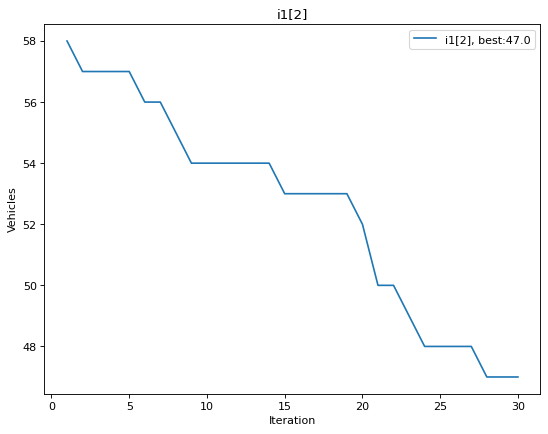
\includegraphics[width=0.8\textwidth]{i1[2]_1_vehicles.png}
\caption{\label{fig:i1[2]_1_vehicles}Time constraint - 1 minute}
\end{figure}

\begin{figure}
\centering
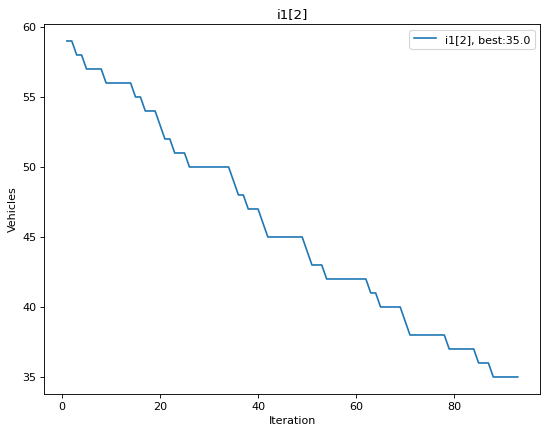
\includegraphics[width=0.8\textwidth]{i1[2]_5_vehicles.png}
\caption{\label{fig:i1[2]_5_vehicles}Time constraint - 5 minutes}
\end{figure}

\begin{figure}
\centering
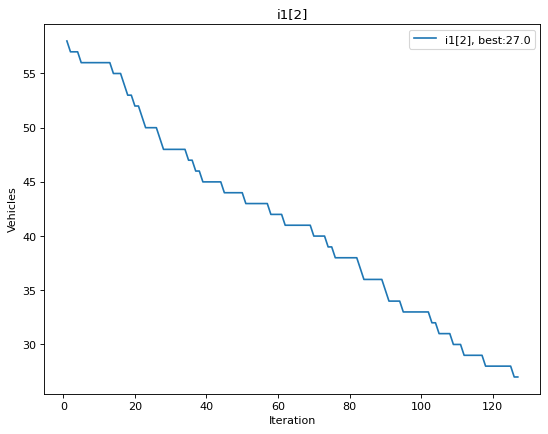
\includegraphics[width=0.8\textwidth]{i1[2]_360_vehicles.png}
\caption{\label{fig:i1[2]_360_vehicles}Time constraint - 6 hours}
\end{figure}

\begin{figure}
\centering
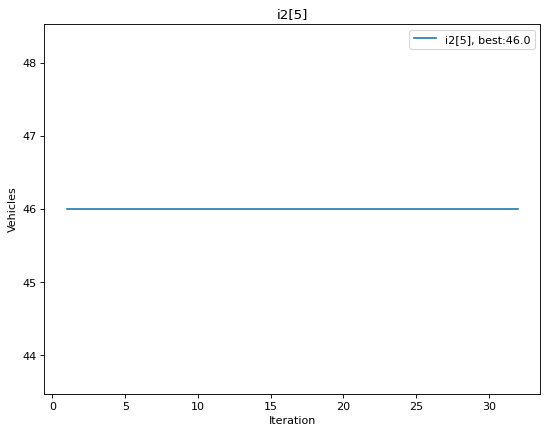
\includegraphics[width=0.8\textwidth]{i2[5]_1_vehicles.png}
\caption{\label{fig:i2[5]_1_vehicles}Time constraint - 1 minute}
\end{figure}

\begin{figure}
\centering
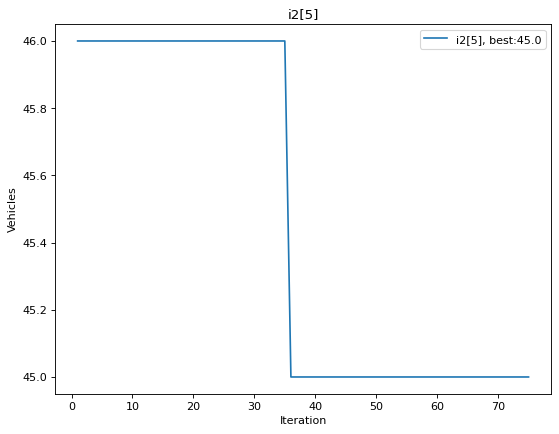
\includegraphics[width=0.8\textwidth]{i2[5]_5_vehicles.png}
\caption{\label{fig:i2[5]_5_vehicles}Time constraint - 5 minutes}
\end{figure}

\begin{figure}
\centering
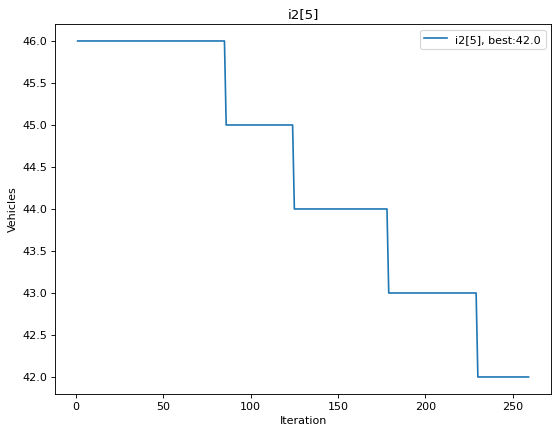
\includegraphics[width=0.8\textwidth]{i2[5]_360_vehicles.png}
\caption{\label{fig:i2[5]_360_vehicles}Time constraint - 6 hours}
\end{figure}

\begin{figure}
\centering
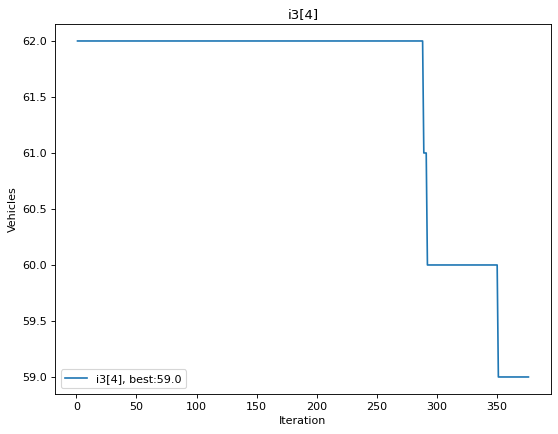
\includegraphics[width=0.8\textwidth]{i3[4]_1_vehicles.png}
\caption{\label{fig:i3[4]_1_vehicles}Time constraint - 1 minute}
\end{figure}

\begin{figure}
\centering
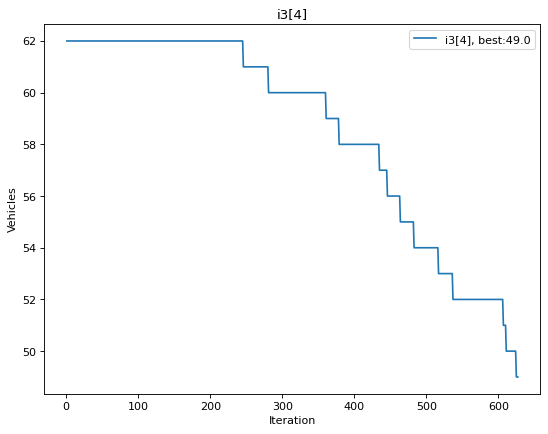
\includegraphics[width=0.8\textwidth]{i3[4]_5_vehicles.png}
\caption{\label{fig:i3[4]_5_vehicles}Time constraint - 5 minutes}
\end{figure}

\begin{figure}
\centering
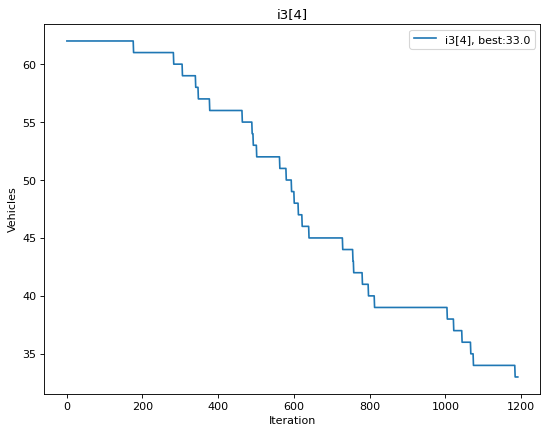
\includegraphics[width=0.8\textwidth]{i3[4]_360_vehicles.png}
\caption{\label{fig:i3[42]_360_vehicles}Time constraint - 6 hours}
\end{figure}

\begin{figure}
\centering
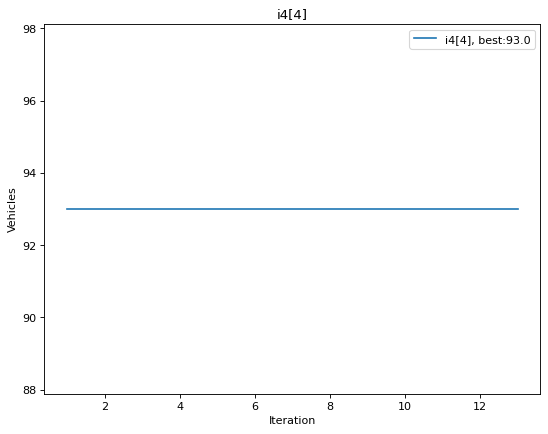
\includegraphics[width=0.8\textwidth]{i4[4]_1_vehicles.png}
\caption{\label{fig:i4[4]_1_vehicles}Time constraint - 1 minute}
\end{figure}

\begin{figure}
\centering
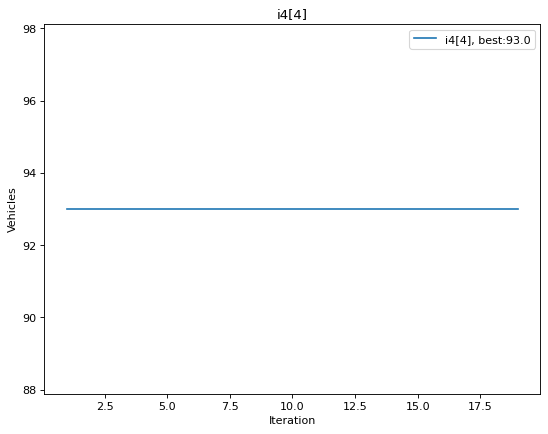
\includegraphics[width=0.8\textwidth]{i4[4]_5_vehicles.png}
\caption{\label{fig:i4[4]_5_vehicles}Time constraint - 5 minutes}
\end{figure}

\begin{figure}
\centering
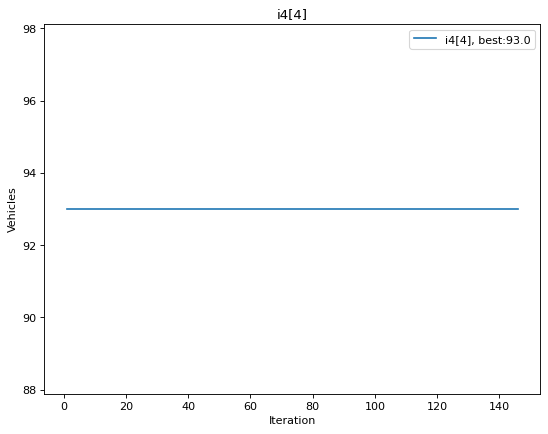
\includegraphics[width=0.8\textwidth]{i4[4]_360_vehicles.png}
\caption{\label{fig:i4[4]_360_vehicles}Time constraint - 6 hours}
\end{figure}

\begin{figure}
\centering
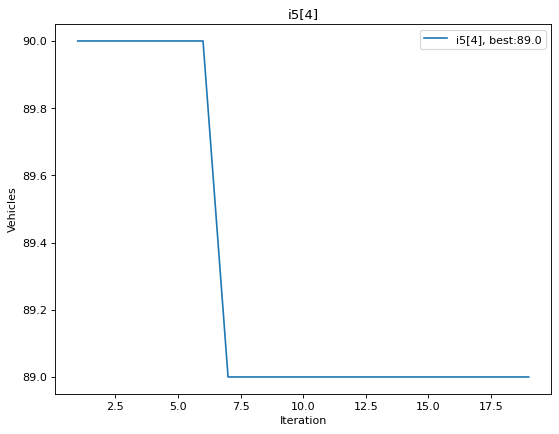
\includegraphics[width=0.8\textwidth]{i5[4]_1_vehicles.png}
\caption{\label{fig:i5[4]_1_vehicles}Time constraint - 1 minute}
\end{figure}

\begin{figure}
\centering
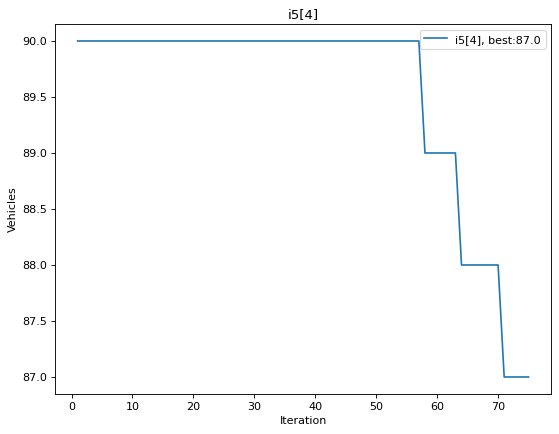
\includegraphics[width=0.8\textwidth]{i5[4]_5_vehicles.png}
\caption{\label{fig:i5[4]_5_vehicles}Time constraint - 5 minutes}
\end{figure}

\begin{figure}
\centering
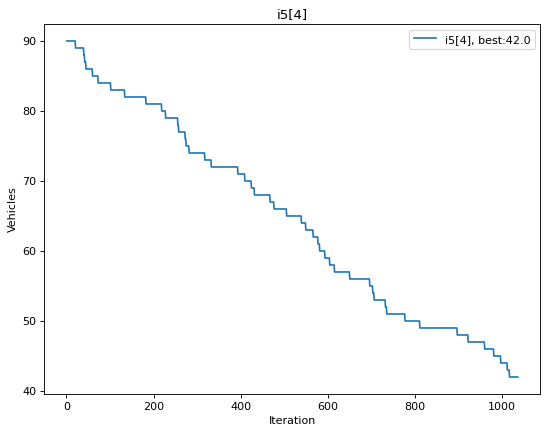
\includegraphics[width=0.8\textwidth]{i5[4]_360_vehicles.png}
\caption{\label{fig:i5[4]_360_vehicles}Time constraint - 6 hours}
\end{figure}

Algorithm used in this project in each instance finds valid solutions. Large Neighbourhood Search performs better when number of customers matches capacity, while it struggles when number of customers increases without increment in capacity.

\clearpage

\section{Conclusion}
The CVRPTW problem involves finding routes for a fleet of vehicles to serve customers while considering capacity and time window constraints. A greedy algorithm was used for the construction phase and a large neighbourhood search was used for local search. The large neighbourhood search improves the solution by randomly removing and reinserting customers into different routes, but it performs better when the number of customers is closely matched with the capacity of the vehicles and may struggle with a higher number of customers without a corresponding increase in capacity. The algorithm was able to find valid solutions for each problem instance.



\end{document}